\section{Az új rendszer alaptáblái}
A probléma leírása alapján elkészíthető a táblák nagyvonalú felsorolása, 
elsődleges elnevezése, illetve a bennük tárolandó adatok vázlatos leírása. Ez a 
későbbiek során bővülhet, szűkülhet, a megnevezések változhatnak. A tervezésnek 
ebben a szakaszában még szabatos neveket használunk.
A táblák előzetes felsorolását \aref{tablak-0} táblázat tartalmazza.
A táblák közötti kapcsolatok \aref{tablak0-kapcs0} ábrán láthatók.
\begin{table}[ht!]
\centering
\begin{tabular}{|c|l|}
\hline
\textbf{Tábla neve}&\textbf{Tartalma}\\
\hline
FELHASZNÁLÓ & a tervezett rendszer felhasználóinak adatai\\
\hline
SZEREP & felhasználói szerepek felsorolása\\
\hline
DOLGOZÓ & dolgozói törzsadatok\\
\hline
KÖLTSÉGHELY & költséghelyek felsorolása\\
\hline
CIKKTÖRZS & mérőeszközök általános tulajdonságai\\
\hline
MŰSZER & mérőeszközök egyedi tulajdonságai\\
\hline
NYILVÁNTARTÁS & melyik eszköz melyik dolgozónál volt, van\\
\hline
KALIBRÁLÁS & kalibrálási adatok\\
\hline
MINŐSÍTÉS & a minősítések felsorolása\\
\hline
FELJEGYZÉS & műszerekhez tartozó feljegyzések\\
\hline
NAPLÓ & a műveletek naplója\\
\hline
\end{tabular}
\caption{Az új rendszer alaptáblái}\label{tablak-0}
\end{table}
\\

\begin{figure}[ht!]\label{tablak0-kapcs0}
\centering
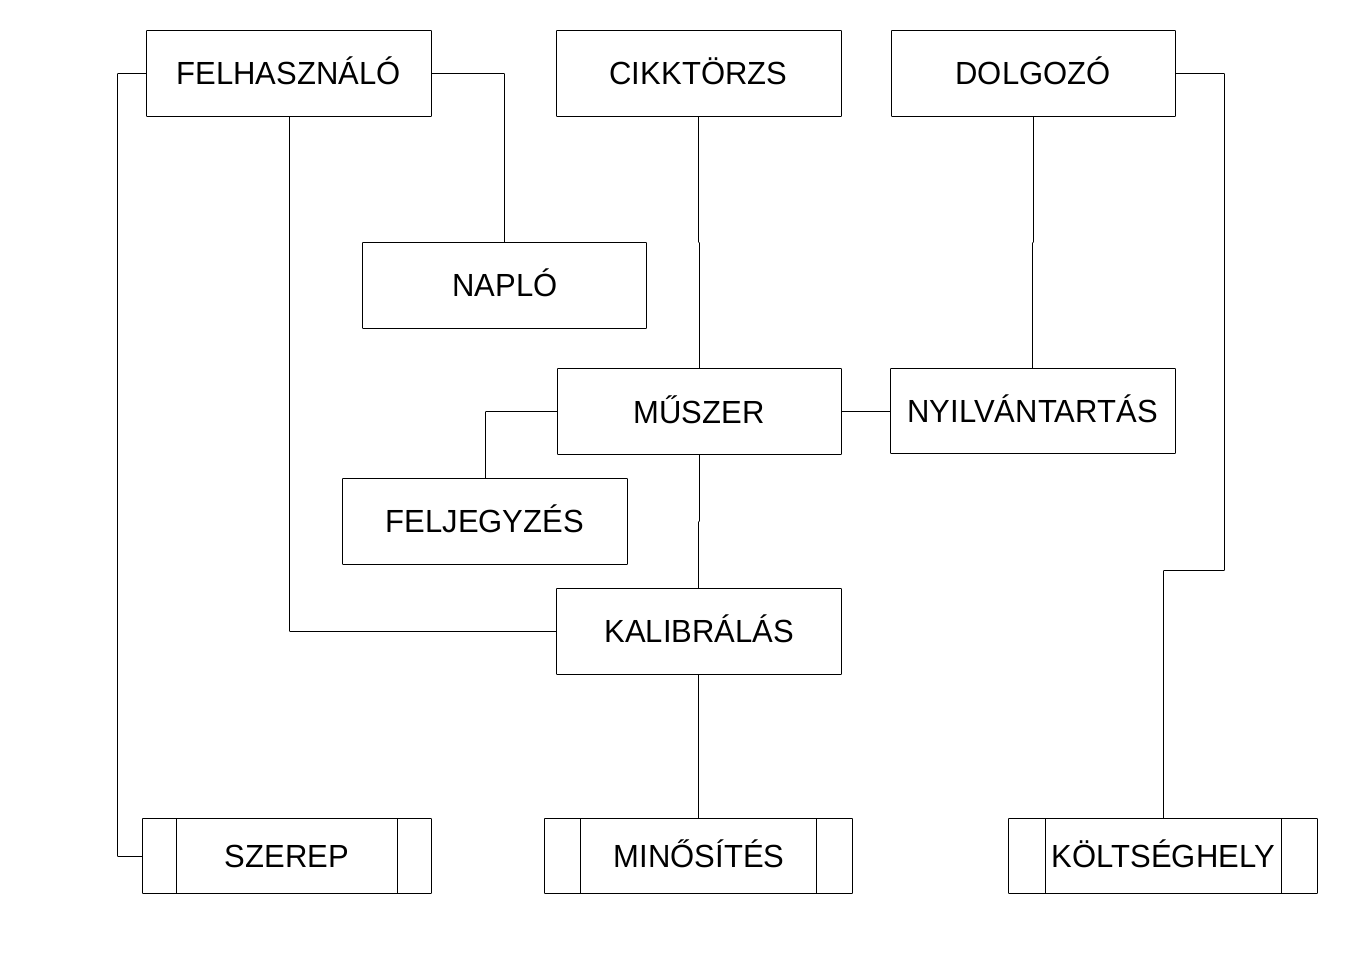
\includegraphics[width=13cm]{kepek/tablak0-kapcs0.png}
\caption{A táblák és a közöttük lévő előzetes kapcsolatok}
\end{figure}

A kapcsolatok ábrázolásánál most még nem foglalkozunk azzal hogy a kapcsolat 
kötelező-e, vagy opcionális, csupán jelezzük, hogy a táblák között van 
valamilyen kapcsolat. Nem jelezzük a kapcsolat fokát, ami lehet \textbf{1:1, 
1:n, m:n} sem.